\documentclass[a4paper,12pt]{book}
\usepackage[utf8]{inputenc}
\usepackage{graphicx}
\usepackage{todonotes}
\usepackage{cite}
\usepackage{subcaption}
\usepackage{amsmath}s

\begin{document}

\author{Christof Backhaus}
\title{Minimum levels of high energy particle bombardment on fusion reactor vessels:\\ \large{Towards a computational multi-parameter scan for automated data reduction ("big data") applications}}
\date{February 2020}

\frontmatter
\maketitle
\tableofcontents
%Abstract
%Introduction
%	Baysian Statistics
%	Gaussian Process Regression
%	Neural Networks
%	NNGP?
%Model description
%	Mitja Beckers Model + Parameter space
%Data Generation
%	low discrepency 

\mainmatter
\chapter*{Abstract}

\chapter{Introduction}
	The design process for a facility like a fusion power plant takes into account a manifold of aspects. Thereunder a cost analysis for the fusion device. To make an estimate of the cost analysis one has to consider the lifetime of machine parts. Most prominently the divertor and first wall suffer from shortened life spans due to erosion. Which is partly due to neutral particle induced sputtering.\\
	To include considerations like these in the design of a power plant one uses so called systems codes like PROCESS\cite{process}. These codes focus on optimizing design parameters of large scale systems like power plants, which consinst of many smaller subsystems. Due to the amount of subsystems the need arises to simplify simulations to achieve reasonable run times for systems codes. The following work is concerned with deducing a fast surrogate in place of a simulation for the sputtering rate of a fusion device component.\\
	The following chapter gives a brief overview of the motivating applications while also introducing the concept of reduced model approaches via machine learning algorithms. Furthermore it considers which methods are most applicable in the given situation.\\
	
	\section{PROCESS Systems Code}
	%TODO Elaborate on difference in point of view: Engineering + marketing vs. Scientific Simulation
	The systems code PROCESS\cite{process} is concerned with the 
	
	%TODO 
	%TODO Example 
	
	\section{Fusion Devices}
	
	%TODO Picture of fusion device
	%TODO Elaborate on difficulty of fusion device longevity
	
	\section{Reduced Model Approaches}

\chapter{Model}
	\section{EIRENE 1D}
		% Mitja Beckers
		%\subsection{Point source}
		%\subsection{Volume source}
		\subsection{Kinetic Boltzmann Equations}
	\section{Plasma Profiles}
		For the inputs of Eirene plasma profiles are needed, that can be dynamically provided by other algorithms like SOLPS\footnote{Citation needed} or EMC3\footnote{Citation needed}. Central piece of this work is to investigate if a substitute function can be found for the full range of possible plasma profiles by using big data methods. One can ascertain the physical limits of the parameters constituting the plasma profiles from table \ref{Par_Bounds}. These limits are based on different phenomenons in plasma physics, which can be 
	\section{Choice of sampling set}
		Since the parameter space is high dimensional, the training points have not been selected randomly. According to \footnote{Add reference} randomly sampled points might form clusters, which could skew the training towards a subsection of the parameter space. To avoid this a low discrepancy sequence, namely the Sobol sequence, has been chosen from which the training points are sampled.
		%\missingfigure{Clustering of points sampled from equal distribution}
		\subsection{Sobol Sequence}
			The sobol sequence was first invented by the mathematician Ilya M. Sobol\footnote{Add citation} 
			\subsubsection{Low-discrepency sequences}
\chapter{Methods}
	\label{Chap:Methods}
	This chapter is concerned with introducing the methods used to investigate the data reduction of the previously introduced model. The focus of this work will be on artificial neural networks (ANN in short) and Gaussian processes.
	The following list will provide a brief overview of other machine learning techniques that are frequently employed in machine learning approaches:
	\begin{itemize}
		\item Support Vector Machines (SVM) \cite{SVMBook}:\\
			%Support Vector Machines
			SVMs are used to classify data similar to ANNs. In contrast to ANNs SVMs are build up from theory and contain little Hyperparameters\footnote{Please refer to section \ref{HyperPar} for further information.} making them easier to analyse and less prone to overfitting. Generally speaking a SVM tries to separate data by calculating a hyperplane using given training data. The separation has a margin\footnote{Area around separation plane that contains no data.} that is maximized. Classification of SVMs are based on which side of the separation the data point lies. For non-linear classification the kernel trick\footnote{A detailed explanation can be found at \cite{KernelTrick}} can be used to create a high dimensional feature space.
			Better suited for classification tasks. Could be used in future endeavours to assess the viability of a certain configuration by classifying input toward a threshold value.\\%, e.g. Sputter rate for first wall lower than X \todo{What is X?}\\
			There are variations of regression SVMs which are difficult to optimize for performance since SVMs rely on analytically calculating the separating hyperplane.\\
		\item Random Forests :\\
			Random forest are ensembles of decision trees, hence the name forest. Each individual tree provides a classification prediction. The class with most votes is prediction of the random forest.\\
			A forest with many uncorrelated trees outperforms highly correlated forest. Random forests have good predictive performance, but slower prediction time which makes them unsuited for system codes.\footnote{A more detailed introductory text can be found at \cite{RandForest}}
		\item Adaptive Boosting:\\
			Not unlike random forests AdaBoost works with an ensemble of decision trees, though in contrast the decision trees used are single split trees called stumps. When training an AdaBoost algorithm the algorithm boosts weights of individual stumps based on their contribution to difficult to classify instances.\footnote{A more detailed introductory text can be found at \cite{AdaBoost}}
%			\begin{enumerate}
%				\item "The weak learners in AdaBoost are decision trees with a single split, called decision stumps.\\				
%				AdaBoost works by putting more weight on difficult to classify instances and less on those already handled well.\\				
%				AdaBoost algorithms can be used for both classification and regression problem."\\
%				\item Adaptive Boosting combines weak classifiers\footnote{Here Stumps, which are very simple decision trees. Basically one feature classifier} into strong classifiers by using weighted sums. Adding new weak classifiers improves the ensemble as long as new classifiers are better than random guesses. If new classifiers perform better on instances that were problematic before than it is added with a higher weight.\footnote{The improvement of the classical Boosting method to the adaptive Boosting (AdaBoosting) won the Gödel Prize in 2003}
%			\end{enumerate}
	\end{itemize}
	\section{Neural Networks}
		The following section is concerned with discussing neural networks as a means of investigating functional dependencies.\footnote{To aid with understanding the terminology used there is a glossary in the appendix section \ref{Glossary}.}\\		
		\subsection{General Introduction To Neural Networks}
		%Definition
			An artificial neural network (ANN) in the following called neural network, abbreviated to NN, is "a computing system made up of a number of simple, highly interconnected processing elements, which process information by their dynamic state response to external inputs." \cite{NNPrimer} %\todo{cite: In "Neural Network Primer: Part I" by Maureen Caudill, AI Expert, Feb. 1989}\\
		% Historical Context, First Introduction, Basic idea
			First concepts of learning processes based on neural plasticity have been introduced in the late 1940s by D. O. Hebb\footnote{Hebbian theory from the neuroscientific field \cite{DOHebb}.}. In 1975 backpropagation became possible via an algorithm by Paul J. Werbos \cite{PJWerbos}, this led to an increase in machine learning popularity. During the 1980s other methods like support vector machines and linear classifiers became the preferred and/or dominating machine learning approach. With the rise in computational power in recent years neural networks have gained back a lot of popularity.\\
			The concept idea of neural networks is to replicate the ability of the human brain to learn and to adapt to new information. The structure and naming convention reflect this origin.\\
		%Structue: Requirements, Deep networks
			A neural network is made up of small processing units called neurons. These are grouped together into so called layers. Every network needs at least two layers, the input layer and the output layer. If a network has intermediary layers between input and output, they are called hidden layers. A network with at least two hidden layers is called a deep neural network (DNN). The amount of layers in a network is called the depth of the network. While the amount of neurons in a layer is called the layers width.
		%As mentioned above the neurons are highly interconnected. The structure of connections determine the type of network. In the following we will discuss fully connected networks\footnote{Fully connected networks are also called dense networks.}. These feature a connection between each neuron of adjacent layers\footnote{The amount of connections between two layers in a dense network is therefore equal the the product of the width of adjacent layers.}
		%Basic working principle, introduced non-linearity
			In a typical NN information stored in neurons is transferred into the next layer by a weighted sum. The connected neuron of the following layer then applies a non-linear function, called activation function, to calculate it's final value. This process in repeated until the output layer is reached. The activation function as well as the amount and interconnectivity of connections can vary in between layers. The system according to which a network is designed is called a network architecture. The most important architectures in the following work will be \textit{dense deep feed forward} and \textit{autoencoder}. To give insight into the basic working principle an example neural network is depicted and described in the following section \ref{NNExample}.\\
			~\\
		%\todo{General description of NN use-cases and strength compared to "old" machine learning methods such as support vector manchines.}
		%Generally speaking neural networks are used to solve the equation $f(x) = y$ for $f()$. In other words it is used to make a fit to data points. There are many already established well known methods to do so. Therefore it is natural to ask what the advantages and disadvantages of neural networks compared to more traditional fitting methods are. To contrast neural networks we will consider support vector machines and analytical fits.
			Neural networks are usually used in two ways, optimization or classification. Well known examples are handwriting recognition as classification and least mean squares (LMS) optimization. %Think of better example for optimization
		\subsection{Functionality}
			\label{NNExample}
			
			\begin{figure}
				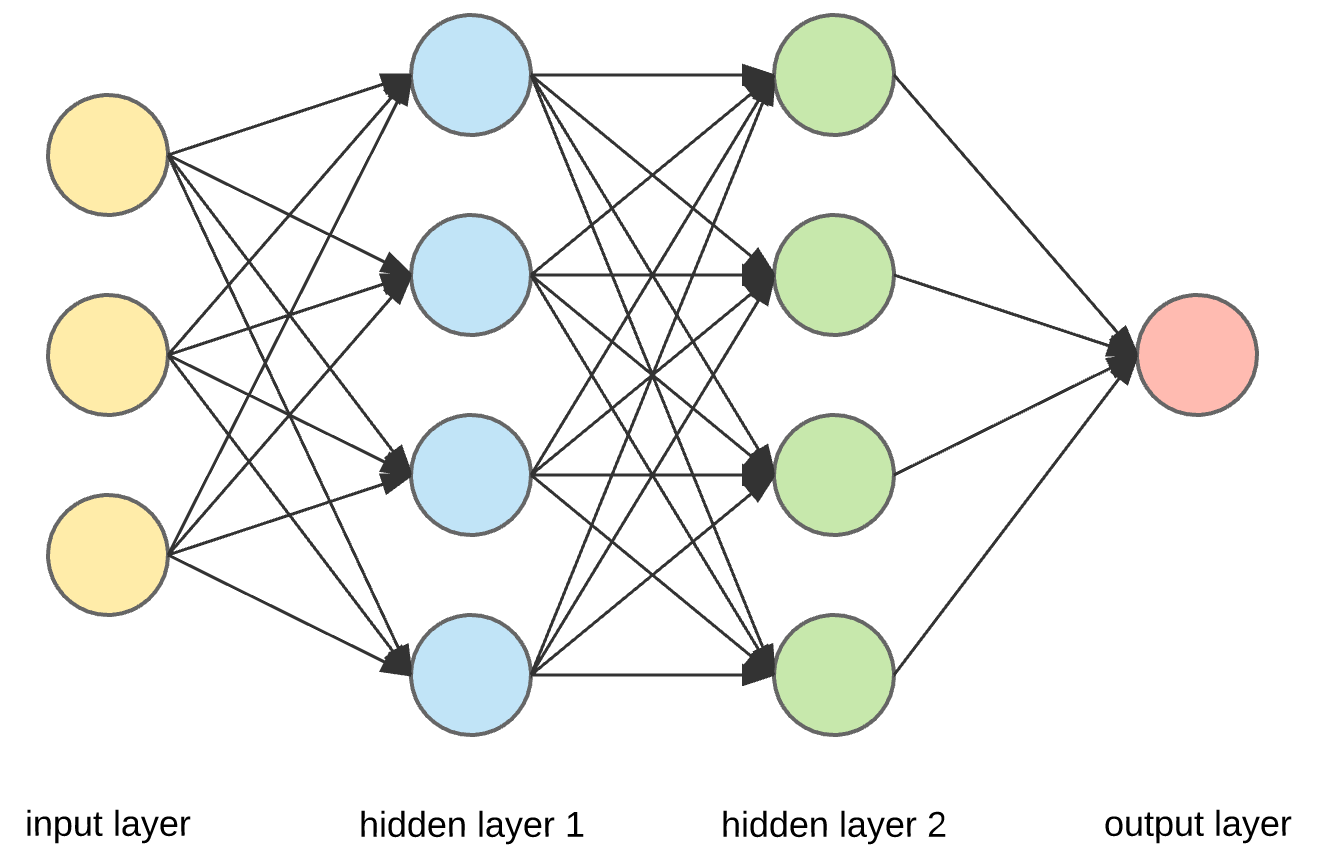
\includegraphics[width=\textwidth]{images/simpleNN.png}
				\caption{Schematic structure of the most basic fully connected deep neural network. Indicated are the input (yellow), output (red) and hidden layers (blue and green). Each neuron outputs to all neurons in the following layer, but there are no interconnection between neurons of the same layer. Note that while the network has the minimum depth (2 hidden layers) to qualify for a deep neural network, the width  could be smaller.}
				\label{Img_NNFully}
			\end{figure}

			%\todo{Funktionsweise}
			The working principle is to form a weighted sum $\sum_{k=1}^{N} w_{j,k} \cdot x_{k}$ over the values from neurons of the previous layer $\vec{x}$ weighted by the connecting weight, elements of the weight matrix $\matr{w}$. The weighted sum is then evaluated by the activation function\footnote{An example activation function is the rectified linear unit function which is depicted in figure \ref{Fig:ReLU} and discussed greater detail in section \ref{Sec:Activation}} $\sigma(x_{k}, w_{j,k}, b_{j})$, with bias $b_j$ such that the new value $x_j = \sigma(\sum_{k=1}^{N} w_{j,k} \cdot x_{k} + b_j)$. Here $k$ refers to the index of the neuron in the previous layer and $j$ to the index of the neuron in the current layer.\footnote{The order of indices becomes more intuitive when talking about backpropagation and its matrix notation in section \ref{BackProp}}\\
			Since forming a weighted sum is a linear operation the activation function must be non-linear to enable the network to learn non-linear behaviour. The most common activation functions are the sigmoid function and more recently the rectified linear unit (ReLU) and exponential linear unit (ELU) shown in figure \ref{Fig:ReLUELU}.\\
		
		\subsection{Training}
			%\todo{Describe training cycle}
			Before a neural network can be put to work it needs to be trained. To train a NN a set of training and test data has to be generated. This work uses the afore mentioned Monte Carlo simulations from the EIRENE code.
			The training data consists of input e.g. temperature and density of the plasma and output e.g. the sputtering rate of the first wall. The EIRENE input data is used as input of the network and the sputtering rate is compared to the output of the network via a cost function. Afterwards the weights of the network are adjusted by using backpropagation, which is a method that calculates partial weight derivatives of the output. A more detailed explanation can be found in section \ref{BackProp}.\\
			%\todo{Explain use of batches, Epochs, Regularization}
			\subsubsection{Backpropagation}
				\label{BackProp}
				To talk about backpropagation it is necessary to first set down a notation. In the following $\matr{w}$ dontes the weight tensor, that contains all weight matrices $\matr{w}^l$ of connections between individual layers $l$. The elements of the individual weight matrices $w^l_{j,k}$ will denote the weight of the connection from neuron $k$ in layer $l-1$ to neuron $j$ in layer $l$. Similarly the matrix $\matr{b}$ contains all bias vectors $\vec{b}^l$ of layer $l$ which in turn contain the biases $b^l_j$ to each individual neuron $j$ of layer $l$.\\
				The activation $a^l_j = \sigma(z_j)$ denotes the weighted input $z_j = \left( \sum^{}_{k} w^l_{j,k} \cdot a^{l-1}_k + b^l_j \right)$ evaluated by the activation function $\sigma(\:)$. Finally a cost function $C$ has to be defined to evaluate the output of the network $\vec{a}^L$ and compare it to the true label $\vec{y}$\footnote{If the network has only one output y is a scalar value.} assigned to the data point $\vec{x}$ by the EIRENE simulation. In the context of training a network the label and inputs are given constants, whereas the weights and biases are adjustable. Therefore the cost function is considered to be a function of all weights and biases $C = C(\vec{a}^L) = C(\matr{w}, \matr{b})$.\\
				%Many of the values above can be accumulated into a vector across neurons of a layer, e.g. The biases $b^l_j$ of each neuron in layer $l$ can be merged into the vector $\vec{b}^l$.
				Shortening the weights notation of $w^l_{j,k} \cdot a^{l-1}_k$ to $\matr{w}^l \cdot a^{l-1}$ with Einstein convention for index $k$ applied.\footnote{This description closely follows chapter 2 of \cite{NNEBook}}\\
				This leads to the vector notation:
				\begin{equation}
					\vec{a}^l = \sigma(\vec{z}^l) = \sigma(\matr{w}^l \vec{a}^{l-1} + \vec{b}_l)
					\label{EQ:Activation}
				\end{equation}
				The backpropagation algorithm aims to provide a computational fast way of calculating the partial derivatives \ref{EQ:BPPart1} and \ref{EQ:BPPart2}. 
				\begin{equation}
					\frac{\partial C}{\partial w^l_{j,k}}
					\label{EQ:BPPart1}
				\end{equation}
				\begin{equation}
					\frac{\partial C}{\partial b^l_j}
					\label{EQ:BPPart2}
				\end{equation}
				Before looking at the partial derivatives of the cost function it is necessary to make two assumptions about the cost function $C$.			
				\paragraph{Assumptions of the cost function}
					~\\ The following two assumptions have to be made.
					\begin{enumerate}
						\item The cost function can be written as an average of cost functions for individual training examples.
						\begin{equation}
							C = \frac{1}{n} \sum_{x} C_x
							\label{EQ:CostCond1}
						\end{equation}
						\item The cost function can be written as a function of the outputs $\vec{a}^L$ of the network:
						\begin{equation}
							C = C(\vec{a}^L)
						\end{equation}
						Where $L$ is the number of layers in a network such that the activation $\vec{a}^L$ is the output of the network.
					\end{enumerate}
					A good example for a cost function that fulfils these requirements is the quadratic cost function
					\begin{equation}
						C(\vec{a}^L) = \frac{1}{2} \left\| \vec{y} - \vec{a}^L \right\|^2 = \frac{1}{2} \sum_j \left(y_j -a^L_j \right)^2
						\label{EQ:Cost2}
					\end{equation}
					 Furthermore the partial derivative $\frac{\partial C}{\partial a^L_j} = (a^L_j - y_j)$ is known and easily evaluated. 
			\paragraph{Backpropagation algorithm}
				A few  more intermediate steps are necessary:
				\begin{enumerate}
					\item Define the error $\delta^l_j \equiv \frac{\partial C}{\partial z^l_j}$.
					\item Start with the error of the output layer\footnote{$\sigma'$ denotes the derivative of the activation function $\frac{\partial\sigma}{\partial z}$}: 
					\begin{equation}
						\delta^L_j = \frac{\partial C}{\partial a^L_j}\sigma'\left(z^L_j\right)
						\label{EQ:BPDel}
					\end{equation}
					\item Express $\vec{\delta}^L$ in a matrix equation\footnote{Hadamard prodcut of two vectors $\vec{x}$ and $\vec{y}$ is given by $\vec{x} \odot \vec{y}= x_j \cdot y_j$}
					\begin{equation}
						\vec{\delta}^L = \nabla_a C \odot \sigma'\left(\vec{z}^L\right)
						\label{EQ:BPMat1}
					\end{equation}
					\item Express $\delta^l$ as a function of $\delta^{l+1}$:
						\begin{equation}
							\delta^l = \left(\left(\matr{w}^{l+1}\right)^T \delta^{l+1}\right) \odot \sigma'\left(\vec{z}^l\right)
							\label{EQ:BPMat2}
						\end{equation}
				\end{enumerate}
				Now the partial derivative \ref{EQ:BPPart1} can be expressed as:
				\begin{equation}
					\frac{\partial C}{\partial w^l_{j,k}} = a^{l-1}_k \delta^l_j
					\label{EQ:BPdCdw}
				\end{equation}
				And the partial derivative \ref{EQ:BPPart2} can be expressed as:
				\begin{equation}
					\frac{\partial C}{\partial b^l_j} = \delta^l_j
					\label{EQ:BPdCdb}
				\end{equation}
				Equations \ref{EQ:BPMat1} and \ref{EQ:BPMat2} provide a fast functionality once the components are known. Luckily all $\sigma'(\:)$ and $\frac{\partial C}{\partial a^L_j}$ are known before start of training and all weight matrices $w^{l+1}$ are calculated during forward pass of each training point. Lastly the error $\delta^l$ can be deduced from the following error $\delta^{l+1}$. Hence, as the name suggests, the algorithm works from layer $L$ backward to the first layer $l=1$.\\
				Therefore the main computational cost of backpropagation is to apply the matrix multiplication of $\left(w^{l+1}\right)^T$ to $\delta^{l+1}$. This can be done in a computational efficient manner over multiple training samples called mini-batches.\footnote{For a more detailed explanation and short proofs of equations \ref{EQ:BPMat1} to \ref{EQ:BPdCdb} please refer to \cite{NNEBook}}

			\subsubsection{Choice of optimizer}
				With the partial derivative of the cost function in respect to any given weight and bias it is possible to adjust them. Additionally a learning rate $\eta$ that depends on the type of optimizer used and architecture of the network has to be chosen. A basic optimizer is the first order Gradient Descend. It applies the following formula to update parameters $\theta$:
				\begin{equation}
					\theta_{t+1}=\theta_t - \eta \nabla C(\theta_t)
					\label{EQ:GD}
				\end{equation}
				Where $\theta$ can be any $w^l_{j,k}$ or $b^l_j$ from the previous section \ref{BackProp}.\\
				There are multiple optimization techniques that improve upon gradient descend. A few concepts are briefly mentioned here, but for a more detailed explanation please refer to \cite{NNOpti}:
				\begin{description}
					\item[Mini Batches] Applying a parameter update after each training example will cause fluctuations that can be helpful in finding minima, but also slow the convergence once close to them. On the other hand applying only one update per training set slows the learning rate immensely. It might not even be possible for training sets that are too large to fit in memory at once. To compromise one uses a mini batch system where subsets of training data are accumulated for update steps. Typical mini batch sizes range from 50 to 256 training examples.
					\item[Momentum] Using the gradient descend optimizer it is easy to see that moving along a slope one can imagine a ball rolling down a slope collecting momentum along the way. This is realized by adjusting the weight update with an additional term from the previous update.
					\begin{eqnarray}
						\theta_{t+1} & = & \theta_t - V(t)\\
						V(t) & = & \gamma V(t-1)  + \eta \nabla C(\theta_{t})
					\end{eqnarray}
					Where $\gamma$ is a simple numerical factor to control the size of the momentum. A typical value for $\gamma$ is around $0.9$.\footnote{This factor can be thought of as how many previous time steps influence the current update. See \cite{NNSGD}ef  for more information.}\\
					While this method speeds up learning  it can also lead to overshooting a minimum. To negate the negative effect a method called Nesterov Accelerated Gradient (NAG)\footnote{More details on NAGs can be found at \cite{NNNAG}.} is used, in which a predictive term slows down momentum if the slope changes signs.
					\begin{equation}
						V_{NAG}(t) = \gamma V(t-1) + \eta \nabla C( \theta_t - \gamma V(t-1))
					\end{equation} 
					\item[Adaptive learning rates] Some neurons activate more seldom than others and therefore it makes sense to put more emphasis on updates of infrequently activated neurons by adjusting learning rates of neurons individually. To do so manually is not feasible, but there are methods like the AdaDelta optimizer that utilise a running average $E[g^2_t]$ of past updates to decrease the learning rate of neurons.
					\begin{eqnarray}
					\theta_{t+1} & = & \theta_t - \frac{\eta}{\sqrt{E[g^2_t]+\epsilon}}g_t \\
					E[g^2_t] & = & \gamma E[g^2_{t-1}] + (1-\gamma) g^2_t
					\end{eqnarray}
					Here $g_t = \nabla C(\theta_t)$ is a shorthand for the gradient and $g^2_t$ the square not laplacian. $\epsilon$ is a small positiv number usually on the order of $10^{-8}$.
				\end{description}
				~\\
				The Adaptive Moment Estimation (Adam) optimizer combines adaptive learning rates, momentum and batch application in one optimizer. It is well suited for sparse problems and has been shown to yield fast convergence. It is therefore the optimizer of choice in the following work.
				\begin{eqnarray}
					\hat{m_t} & = & \frac{m_t}{1-\alpha_t}\\
					\hat{v_t} & = & \frac{v_t}{1-\beta_t} \\
					\theta_{t+1} & = & \theta_{t} - \frac{\eta}{\sqrt{\hat{v_t}}+\epsilon}\hat{m_t}
				\end{eqnarray}
				Here $m_{t+1} = \alpha \: m_t + (1-\alpha)g_t$ denotes the mean of the gradient and $v_{t+1} = \beta v_t + (1-\beta)g^2_t$ the variance. $\alpha$ is typically as large as $\gamma$ from AdaDelta, around $0.9$. $\beta$ is close to 1 with a default value of $0.999$. 
			\subsubsection{Regularization}
				From the description above it should be clear that the number of parameters in a neural network can easily exceed the one or even ten thousand, some state-of-the-art neural networks even exceed 40 million parameters\footnote{See \cite{BookMultimediaModeling} page 149} \todo{Search for further references}. With that many parameters a model can fit to nearly any set of data reasonably well. John von Neumann famously said:"With four parameters I can fit an elephant, and with five I can make him wiggle his trunk."\footnote{See \cite{NNElephant}}\\
				The aim of a network is to give accurate predictions on data it has never seen before. Therefore it is critical to ensure the learning gains generalize well to unknown data. Any method that aims to increase prediction accuracy on the test set at a disregard to the accuracy of the training predictions is called a regularization method. Inversely the increase in training accuracy with stagnating or even degrading of test prediction accuracy is called overtraining or overfitting.\\
				In the following we will shortly introduce the most commonly used regularization methods.
				\paragraph{Hold out}%\todo{maybe change to subsubsubsection instead of paragraph}
					In this work training and test sets have been mentioned before. This is the appropriate point to go into a little more depth at why the distinction is necessary. Furthermore a third set called validation set is introduced.\\
					The naming of the three sets is already indicative of what their purpose is.
					\begin{description}
						\item[Training Set] Set of examples used during the training process. The network iterates on these points to adjust weights and biases to minimize the cost function.
						\item[Validation Set] Set of examples used after training to evaluate the performance of the network. After which hyper parameters like architecture or learning rate are reassessed.
						\item[Test set] Set of examples used after hyper parameters have been tuned. Used to judge final performance of the network.
					\end{description}
					At first glance validation and test set seem to fulfil a similar role in that they are used to validate the learning process of the network. Since overtraining is a major concern, it is also important to consider overfitting the hyper parameters. Considering the tuning of hyper parameters as an optimization task to improve test accuracy shows that the validation set really is more similar to the training set on a higher meta-level. Therefore it is necessary to split potential test data into a validation and test set. This allows to have a data set that the network does not see over the training and validation process.
				\paragraph{L1 Regularization}
					Adding an additional term to the cost function that is dependent on the weights forces the network to use small weights. For the L1 Regularization this term is $\frac{\lambda}{n} \sum_{w}^{\,} \abs{w}$ such that the new cost function becomes:
					\begin{equation}
						C = C_0 + \frac{\lambda}{n} \sum_{w}^{\,} \abs{w}
					\end{equation}
					Here $C_0$ denotes the original cost function and $\lambda$ is a hyper parameter called the regularization parameter. The effect of this regularization becomes apparent when considering its partial derivative $\frac{\partial C}{\partial w} = \frac{\lambda}{n} \mathrm{sgn}(w)$ that is used to adjust the weights via backpropagation.\\
					The new update rule becomes:
					\begin{equation}
						w_{t+1} = w_t  - \frac{\eta \lambda}{n}\mathrm{sgn}(w) - \eta \frac{\partial C_0}{\partial w_t}
					\end{equation}
					Subtracting a constant amount drives the weights towards 0. This causes the network to focus on a few high importance neurons which can be an advantage but is not generally a wanted quality. The following L2 Regularization improves upon this idea.
				\paragraph{L2 Regularization}
					From the name and the previous L1 regularization it can be inferred that the L2 regularization adds the following term to the cost function:
					\begin{equation}
						C = C_0 + \frac{\lambda}{n} \sum_{w}^{\,} \| w^2 \|
					\end{equation}
					Which leads to the following update rule:
					\begin{equation}
						w_{t+1} = w_t \left( 1 - \frac{\eta \lambda}{n}\right) - \eta \frac{\partial C_0}{\partial w_t}
					\end{equation}
					Where the L1 regularization shrank each weight by the same amount, the L2 regularization rescales the weights while penalising large weight terms harsher. This leads to many small weights contributing to the network performance. Reducing the size of weights is appealing because large weights can be used to learn single features like particularities of the training data. 
				\paragraph{Dropout}
					Before discussing neural networks there was a brief mention of alternative machine learning methods. Many of which made use of an ensemble of weak classifiers to work together as a strong classifier. Dropout manages to achieve much the same in that it deactivates a portion of neurons randomly selected in each training phase. The remaining neurons form a subnetwork which is tasked with learning the same task as the full size network. Each configuration of neurons or subnetwork can be seen as a weak classifier that when dropout is deactivated for validation perform together as a strong classifier. Furthermore dropout regularizes the network by averaging over the results of the subnetworks. Therefore for a overfitting a feature it has to be learned by multiple subnetworks.
				\paragraph{Data variation}
					As explained overfitting happens when a model has more parameters than data points to fit. Hence procuring more training data would remedy this problem. Data variation provides a method to expand the pool of training examples without the need for new data.\\
					It is more easily explained when thinking of images to classify. A common example is recognition of handwritten numbers. Here a training example is an image of a single digit, which can be streched, rotated or otherwise be transformed and still be recognizable as the same digit. Therefore applying a transformation to the training data allows to multiply the number of available training examples by the amount of transformations applied.\\
					For the task at hand a data transformation can be applied and seen as measurement inaccuracy for the inputs and stochastic inaccuracy of the Monte Carlo data for the output.\footnote{This assumes that the functionality of the underlying model is smooth, which can be seen as given due to the network trying to learn such a smooth function anyways.}\\
					A neat side effect of data variation is that the model becomes more robust to exactly the transformations applied. Again this can be more easily understood in terms of image recognition. For example face recognition software might be able to better recognize reflections if a flip transformation (mirror effect) has been applied to the training examples.
			%\subsubsection{Choice of test data}
				%To validate and test network performance in this work half as many points as for training were chosen via random input variables (between 0 and 1). Then the monte carlo simulation was run and recorded along the corresponding input.
		\subsection{Hyperparameters}
			\label{HyperPar}
			\subsubsection{Activation Functions}
				\label{Sec:Activation}
				When designing a neural network it is important to consider which activation function to use. There are requirements of a suited activation as well as varying advantage of using one or another.\\
				In the past a major problem of neural networks has been vanishing of gradients.\footnote{
				As explained in section \ref{BackProp} in order to adjust the weights it is necessary to calculate the partial derivative of the cost function in respect to each weight. Backpropagation can be done without needing to apply the chain rule to calculate the partial derivatives, but using the chain rule obviously has to yield the same result, if our algorithm is working correctly.\\
				Choosing a sigmoid $f(x)=\frac{1}{1+e^-x}$ as activation function leads to a derivative $f(x)=\frac{e^-x}{(e^-x+1)^2}$ with vanishing values at the fringes. For each layer between the current and the output applying the chain rule will result in a partial derivative factor with values between 0 and 1. Hence in a network with realistic depth e.g. 50, the partial derivative calculated for adjusting the weight will be almost always negligible for the beginning layers.}\\
				To avoid vanishing gradients a better choice than the sigmoid can be found. The most common activation function for neural networks is the rectified linear unit (ReLU), shown in figure \ref{Fig:ReLU}.
				\begin{equation}
					f(x) =
					\begin{cases}
						0 & x < 0\\
						x & x \geq 0
					\end{cases}
					\label{EQ:ReLU}
				\end{equation}
				The derivatives of this function is easily computed to 0 for $ x < 0$ and 1 for $ x \geq 0$. While an activation like the sigmoid function has two sided saturation\footnote{Values at either end of the spectrum have small derivatives.}. The ReLU activation saturates only for negative values, which can be interpreted as neurons that work like switches specialising in detecting certain features, see \cite{VanGrad}. In some networks this is a wanted quality of the ReLU activation.\\
				The downside of saturation, and it's vanishing gradient, whether one or two sided is that once a neuron has reached a saturating value it will change hardly or not at all from it, due to the small or even 0 gradient. This leads to a slow down or stagnation of the learning process.\\
				To alleviate the 0 gradient of the ReLU activation one can introduce a leaky ReLU or Parametric ReLU (PReLU) function. That has a flatter linear part in the negative range:
				\begin{equation}
					f(x) =
					\begin{cases}
						\alpha x & x < 0\\
						x & x \geq 0
					\end{cases}
					\label{EQ:PReLU}
				\end{equation}
				If $\alpha$ is randomly initialized or static the function is called (Randomized) Leaky ReLU. If $\alpha$ is a parameter of the network and improved during training, the function is called PReLU. A typical value for a static parameter according to \cite{VanGrad} is $\alpha = 0.01$.\footnote{Also some works indicate that for a static parameter $\alpha = \frac{1}{5.5}$ is a better choice.}\\
				An even better activation function is the Exponential Linear Unit (ELU), depicted in \ref{Fig:ELU}, which offers a one sided saturation with a monotone and smooth gradient. The downside is that while it performs generally better in terms of accuracy, it is also slower in both training and predictions, since a lot of exponential functions have to be evaluated.\\
				\begin{equation}
				f(x) =
					\begin{cases}
						\alpha (e^x - 1) & x < 0 \\
						x & x \geq 0
					\end{cases}
				\end{equation}
			\begin{figure}
				\begin{subfigure}{.49\textwidth}
					\centering
					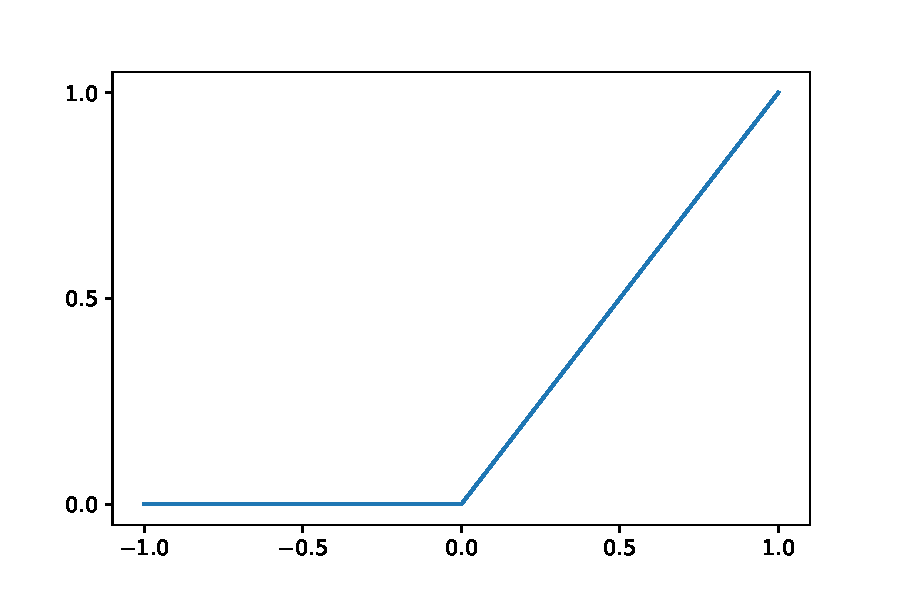
\includegraphics[width=\textwidth]{images/ReLU.pdf}
					\subcaption{Rectified Linear Unit}
					\label{Fig:ReLU}
				\end{subfigure}
				\begin{subfigure}{.49\textwidth}
					\centering
					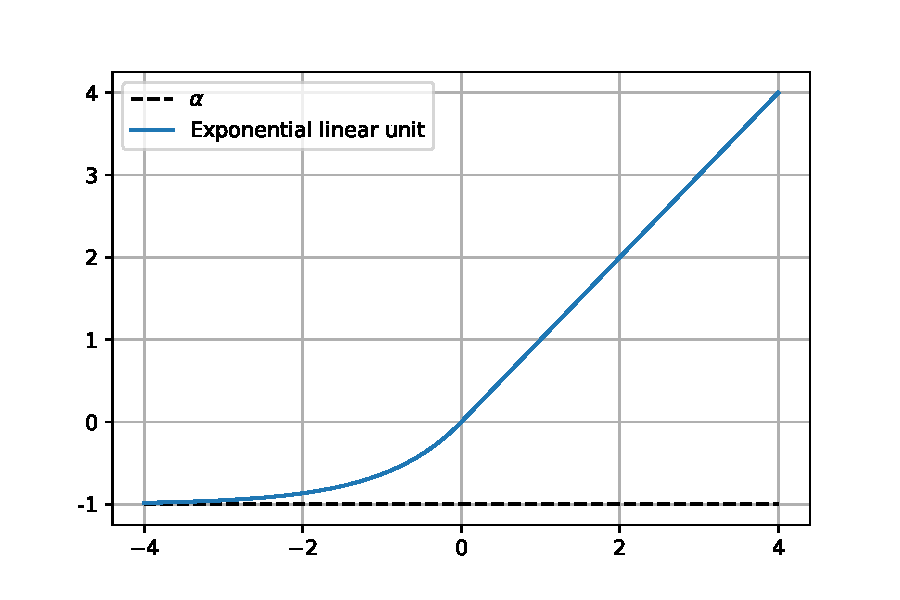
\includegraphics[width=\textwidth]{images/Elu.pdf}
					\subcaption{Exponential Linear Unit}
					\label{Fig:ELU}
				\end{subfigure}
				\caption{Example activation functions rectified linear unit (a) and  exponential linear unit (b) used to introduce non-linearity into neural networks.}
				\label{Fig:ReLUELU}
			\end{figure}
		
		\subsubsection{Architecture}
			The architecture of a network refers to its shape and type of connection. As previously done it is useful to first set down some fundamental terms:
			\paragraph{Depth}
			The amount of layers in a network is referred to as the depth of the network. Commonly the input and output layers are omitted for this count, since they are essential for any network.
			\paragraph{Width}
			The width of a layer refers to the amount of neurons in that layer. Often networks are build of layers with the same width in each hidden layer. If that is the case one speaks of the width of the network.
			\paragraph{Dense layers}
			A fully connected or dense neural network like depicted in figure \ref{Img_NNFully} is characterized by connecting every neuron from the previous to all neurons of the following layer. In contrast to other networks this allows for a very high flexibility but also lacks the spatial context of data. This kind of network is especially well suited for data that is given in form of vectors or drawn from an arbitrary parameter space.\todo{insert reference}
			\paragraph{Feed Forward Networks}
			Any network that propagates information only from input to output is called a feed forward network.
			\paragraph{Recurrent networks} Recurrent networks allow the use of outputs as inputs. They are typically used in speech and text recognition and processing. Recurrent networks excel in contextualizing information. For example recognizing words as part of a sentence structure.
			\paragraph{Autoencoder Networks}
				Autoencoder networks are build symmetrically around a center layer. The output tries to replicate the input instead of a given label. This allows to build a network that simulates a principal component analysis. Looking at the size of the center layer, which is tried to minimize, indicates a set of parameters needed to reconstruct the full information of the input. Hence it allows for dimensionality reduction. This can be used to perform a coordinate transformation of the input data to use for later processing. An example will be shown in the results chapter, section \ref{Res:Auto}.
			\paragraph{Other types}
				There is a wide range of different architectures, some of which can be seen in fig. \ref{Fig:NNZoo}. Most of which are not of further importance to this work, but at least convolutional, probabilistic and spiking networks should be mentioned. Since they excel in their respective fields.
			%\paragraph{Spiking networks} Spiking networks adapt the biological property of a neuron to fire a signal if an inner potential has been reached. To this goal the state of each neuron is described via a differential equation that decays over time and increases if activated by an incoming spike.
			
			\begin{figure}
				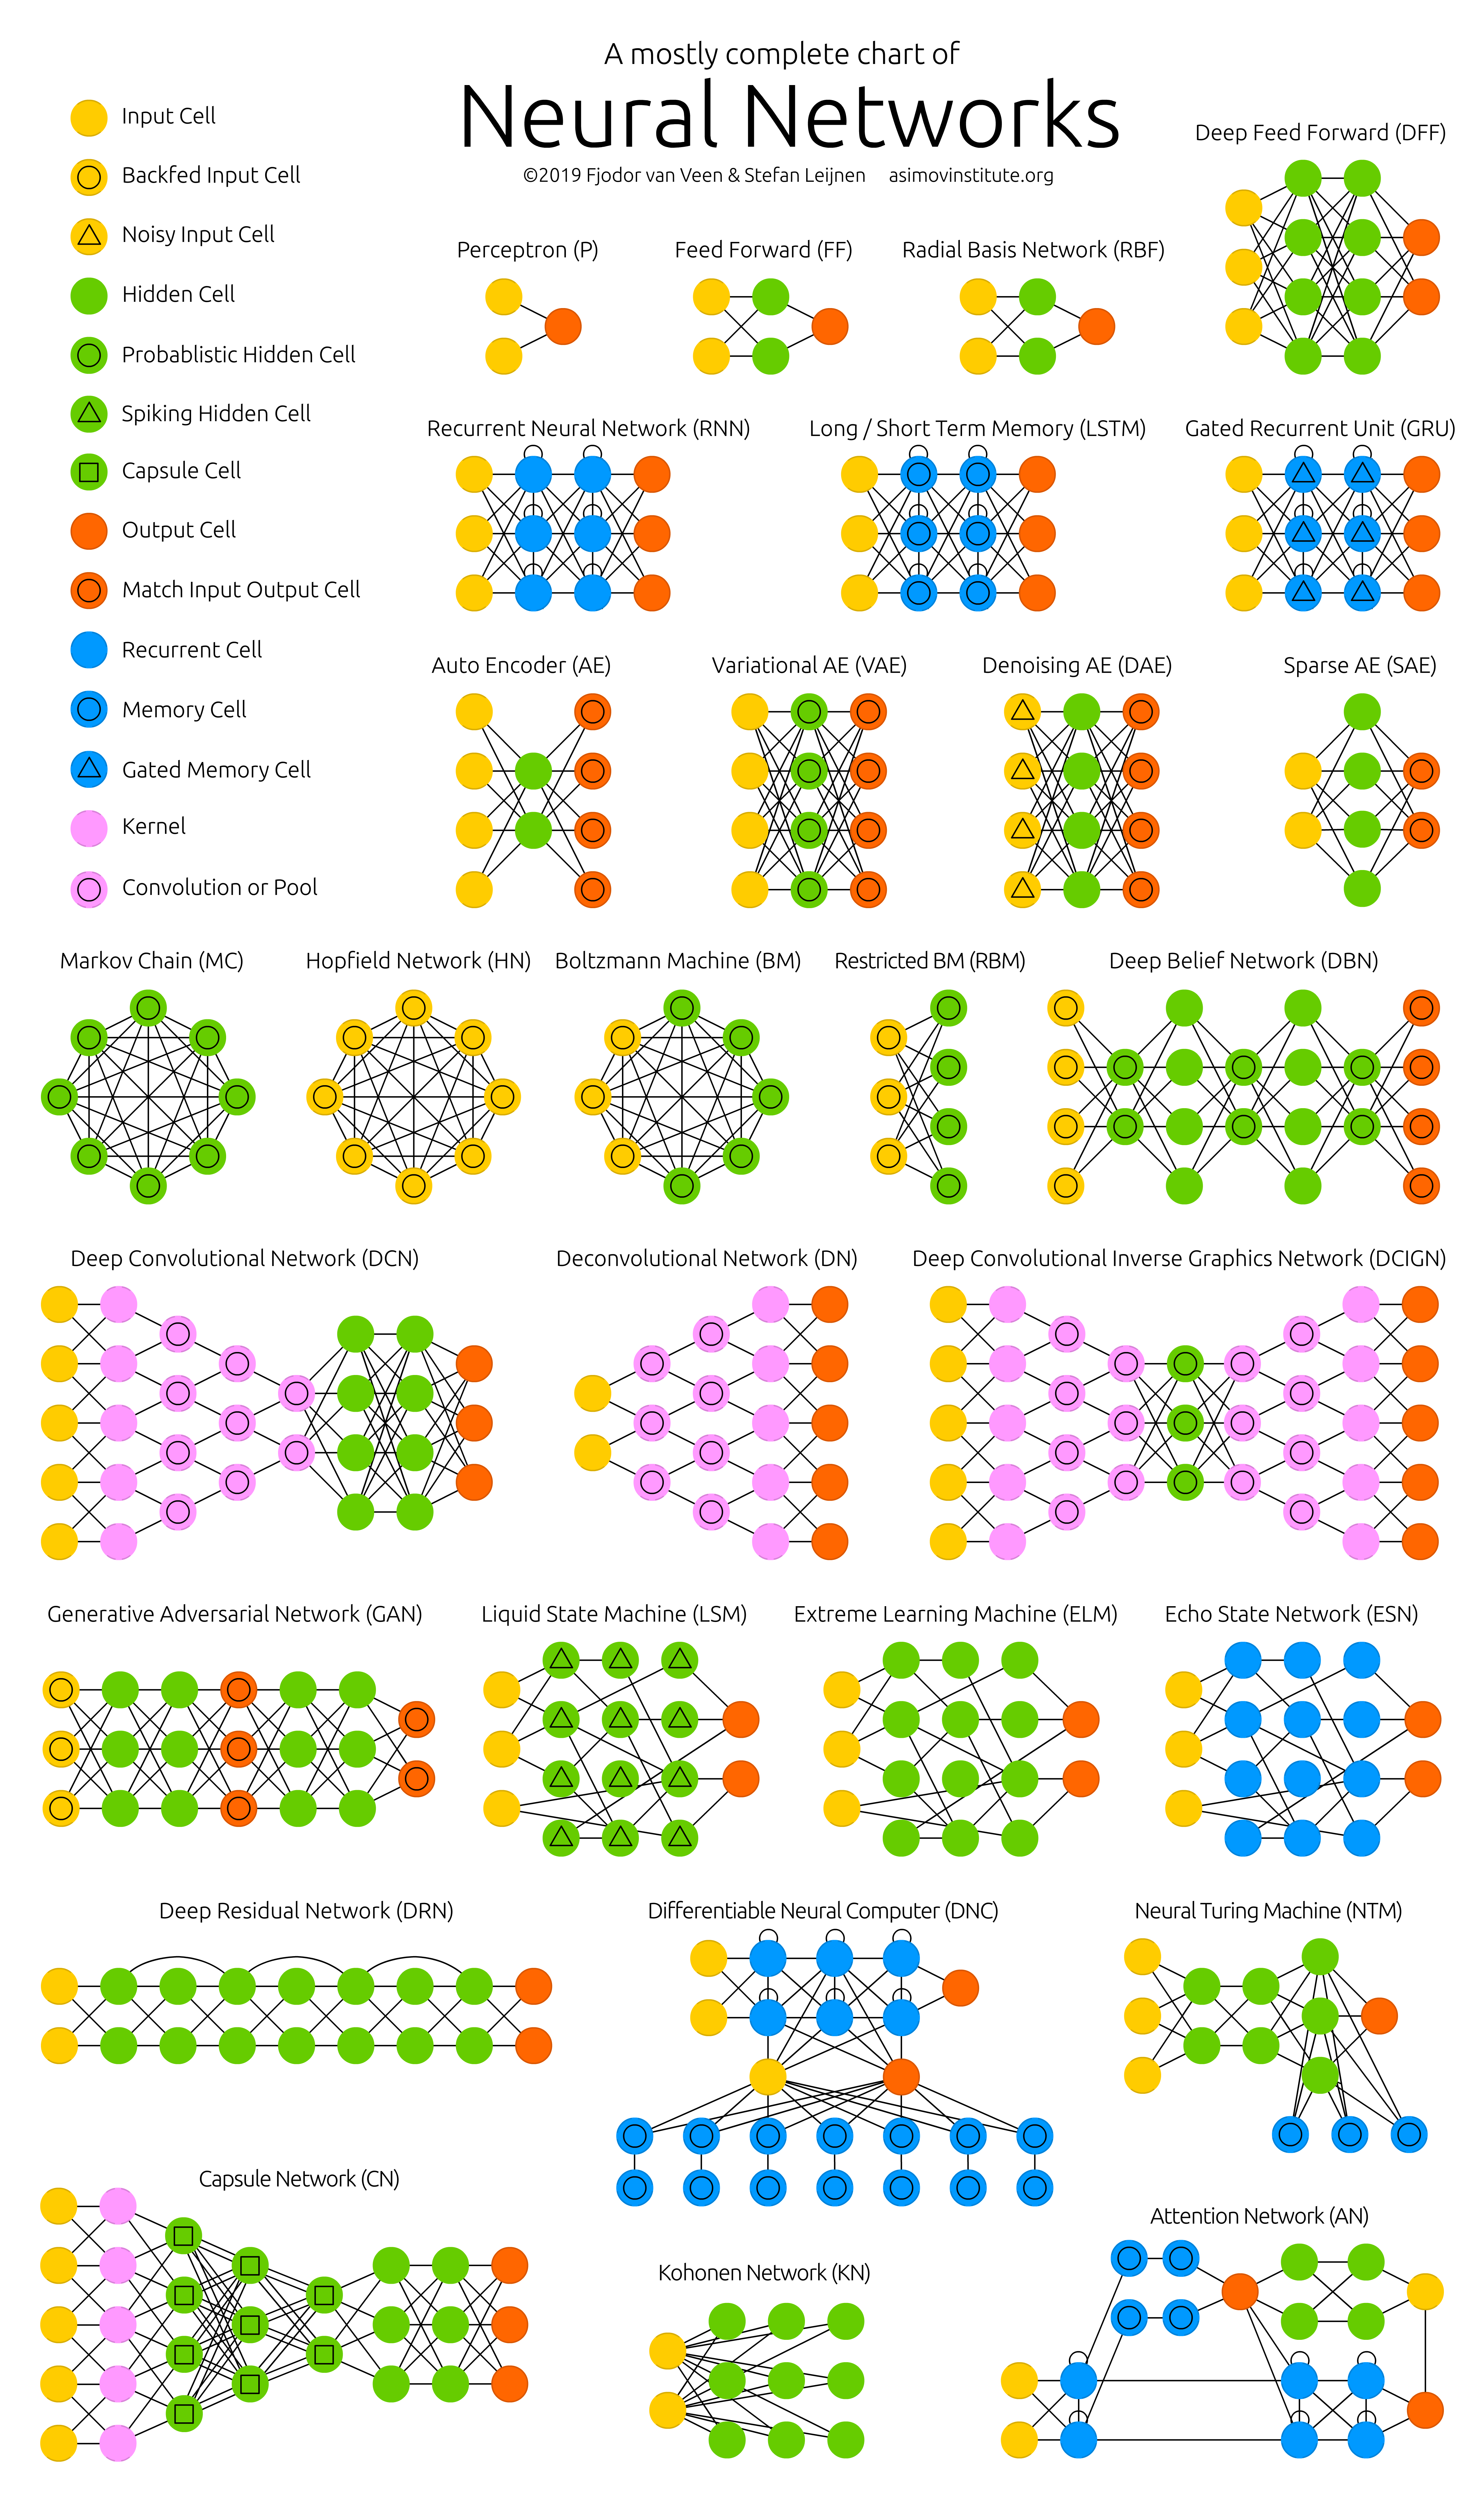
\includegraphics[width=0.8\textwidth]{./images/NeuralNetworkZoo.png}
				\caption{Zoo of Neural network architectures. Image taken from \cite{ImgNNZoo}}
				\label{Fig:NNZoo}
			\end{figure}
		\subsubsection{Cost function}
			The default cost function is the well known mean squared error formula \ref{EQ:Cost2}, that has already been used as an example before. For the more general case of calculating the cost of multiple training examples the it has to be multiplied by $\frac{1}{n}$, where $n$ is the number of examples.\\
			Alternatively the cross-entropy function is used, if the output is on the scale of 0 to 1, which can be easily achieved by using a sigmoid or softmax activation function in the last layer.
			\begin{equation}
				C(x) = -\frac{1}{n} \sum_{x} \left[ y \: \mathrm{ln}(a) + (1-y) \: \mathrm{ln}(1-a) \right]
				\label{EQ:CostCrossEntropy}
			\end{equation}
			Here $n$ is the number of inputs $x$ and corresponding labels $y$, $a$ denotes the activation of the last neuron layer.\\
			The main advantage of the cross entropy function is that its partial derivative to either weights or biases does not depend on the derivative of the activation function, but on the value of the activation function. Thus it prevents slowdown of the learning process.\footnote{See chapter 3 of \cite{NNEBook} for more detail.}
			%http://neuralnetworksanddeeplearning.com/chap3.html
			\begin{eqnarray}
				\frac{\partial C_{\mathrm{quadratic}}}{\partial w} & = & a \sigma'(z)\\
				\frac{\partial C_{\mathrm{cross entropy}}}{\partial w} & = & \frac{1}{n} \sum_{x} x_j (\sigma(z)-y) 
			\end{eqnarray}

			\paragraph{Batch size and Epochs}
				During training an update step can occur after each training example\footnote{This is called stochastic gradient descend.}, after the whole training set has been processed\footnote{This is called batch gradient descend.} or a after a set amount, called batch size, of training examples has been fed to the network. Research\footnote{add citation see comment} suggests that using a small batch size is optimal, but as with many other hyper parameters the exact size depends on the problem and other hyper parameters.\\
				Smaller batch sizes lead to more noisy updates which has a regularizing effect on the network, though it increases computing time, since more updates are made.\\
				An epoch marks the time when every training example has been shown to the network once. At that time the next batches for training are created.\footnote{For example with 100 data points and a batch size of 10, 10 random points are assigned to each batch. Meaning that batches over different epochs contain different training examples.} Epochs are a useful measure of training efficiency. Often training progress is depicted in graphs of epochs against prediction accuracy.
			

						
%	\section{Gaussian Processes}
%		\todo{add citation: Gaussian Processes for Machine Learning (book and website)}
%		\begin{itemize}
%			\item Based on baysian statistics\\
%			\item Definition of Gaussian Process\\
%			\item Use in machine learning
%		\end{itemize}
%		\subsection{Gaussian Process Regression}
%			\begin{itemize}
%				\item usually used for classification\\
%				\item changes to use for regression\\
%				\item limited by inverting of matrix (of input parameters)\\
%				\item better suited for problems with low amount of initial data
%			\end{itemize}
%		\subsection{GOGAP algorithm}
%			Mention
%	\section{NNGP ?}
\chapter{Results}
	\label{Chap:Results}
	%\section{Physical Results}
	\section{Neural Networks}
		The following subsets of hyper parameters have been investigated:
		\subsection{Architecture}
			To begin with a general analysis of the architecture is performed. All architectures tested in this section, have been tested with the maximum amount of data to ensure the best possible learning process. Furthermore they have been validated and tested using $2^{15}$ data points each. Due to assumptions of best suited hyper parameters as explained in chapter \ref{Chap:Methods} section \ref{HyperPar}, the initial layer of neurons uses a sigmoid activation function followed by LeakyReLU layers and the output layer has a linear activation function. Dropout has been set to 0.4, the loss function is Root-Mean-Squared and the optimizer is Adam with NAG-momentum and decay. All of these parameters can be found in table \ref{Tab:ArchPar}.\\
			\begin{tabularx}{\textwidth}{c|c|X}
				Parameter & Value & Note\\
				\hline
				Number of Training Points & $2^{17}$ & Sobol Points to ensure coverage of parameterspace\\
				Number of Validation Points & $2^{15}$ & Points Randomly sampled from Parameterspace \\
				Number of Test Points & $2^{15}$ & Randomly sampled from Parameterspace\\
				Optimizer & Adam & $\alpha = 0.001$, $\beta_1 = 0.9$, $\beta_2 = 0.999$, $\epsilon = 10^{-8}$, \\
				Loss Function & RMS & \\
				Activation function & Leaky ReLU & $\alpha = 0.2$\\
				Batch size & $2^{14}$ & 8 Batches per Epoch\\
				Maximum Epochs & $1000$ & Early Stopping with patience 50, monitoring validation loss\\
			\end{tabularx}
			
			\begin{figure}
				\centering
				\includegraphics[width=\textwidth]{../Data/Results/Choice/Architecture.pdf}
				\caption{Neural network architectrue with best training performance at maximum scale, without fine tuning.}
				\label{Fig:ResArch}
			\end{figure}
			
			\begin{tabularx}{\textwidth}{c|c|X}
				Shape & Test Loss & Note \\
				\hline
				Evenly spaced & 3.547966 & \\
				Triangular & 0.971974 & \\
				Reversed Triangle & 0.895224 & \\
				Hourglass & 3.320479 & \\
				Centered & 1.021901 & \\
				Stretched Centered& 0.986 & \\
			\end{tabularx}
			Figure \ref{Fig:ResArch} shows the typical progression of the learning process of a neural network. The blue curve shows the training loss as training progresses. The orange curve shows the validation loss and the black line the test loss. The test loss is just a scalar value since the test evalutaion of the network is done after the training is completed.\\
			It is expected that the training loss has the lowest value followed by the validation loss and the test loss being highest. That being said the expectation is that the test and validation loss are very close.\\
			Initially training and validation loss might be very high due to random initialization of weights. That can also lead to bad learning behaviour, which is why all architectures have been tested multiple times to reduce the influence of bad initialization. Also the initialized weights are he-normalized.\\
			Due to dropout the training loss stays above the validation loss. Showing that the subnetworks formed in training are not able to adequately adapt the underlying behaviour. Giving rise to investigate the influence of the droprate parameter and additionally tuning the batch size to allow the subnetsworks to better adapt during training.\\
			All tested architectures followed the trend as shown in figure \ref{Fig:ResArch}. None showing a systematic plateauing or significantly better or worse training behaviour.\\
			It is surprising to see a much worse value in testing than in validation, since both validation and test data have been sampled from the same random distribution. Hence it would be expected that both have similar values. Especially since no finetuning of the network has been done that would explain a lowered validation loss.\todo{Test with validation and test set switched.}
			
			\begin{figure}
				\centering
%				\includegraphics[width=\textwidth]{}
\missingfigure{Here will be a nice figure}
				\caption{}
				\label{key}
			\end{figure}
		
			With the general structure locked into place the next test series is used to investigate how the size of the network impacts performance, based on the assumption that a larger network will have better adaptation and hence precision, but takes more time to train, evaluate and make predictions. At first the depth of the network is kept the same while the width is varied, afterwards the width is kept constant. Lastly a test series with about constant amount of weights is done. The Results can be found in tables \ref{Tab:CDepth}, \ref{Tab:CWidth}, \ref{Tab:CPara}.
			
			\begin{tabularx}{\textwidth}{c|c}
				Depth & Test Loss\\
				\hline
			\end{tabularx}
			\begin{tabularx}{\textwidth}{c|c}
				Width & Test Loss\\
				\hline
			\end{tabularx}
			\begin{tabular}{c|c|c|c}
				Number of Total Parameters & Depth & Width & Test Loss \\
				\hline
			\end{tabular}
			\paragraph{Conclusion} After these tests we can conclude that for the given datastructure and problem the most optimal structure is: \todo{Summarize final architecture}.

		\subsection{Training Set Size}
			Depth and Width together determine the total number parameters and complexity of the network. The question is how complex does the network needs to be to accurately learn the model. Ideally we'd like to trim the network as much as possible without loosing too much accuracy.\\
			\begin{tabular}{c|c|c}
				Number of Training Points & Number of Validation Points & Number of Test Points\\
				\hline
			\end{tabular}
			\subsubsection{Activation}
				\begin{itemize}
					\item ReLU \\
					\item PReLU \\
					\item ELU \\
					\item Conclusion
				\end{itemize}
			\subsubsection{Optimizer}
				\begin{itemize}
					\item SGD with momentum\\
					\item Adam 
				\end{itemize}
		\subsection{Derivatives}
%	\section{Gaussian Processes}
%		\subsection{Subdivion of parameter space}
%		\subsection{Derivatives}
%	\section{Comparison}
%		\subsection{Accuracy}
%	\section{NNGP - Maybe}
\include{./TeX_files/conclusion}
\appendix
\chapter{More Data probably}
\chapter{Background Neural Network}
	\section{Overview of Hyper parameters}
	A hyper parameter refers to a parameter of the network that is not changed during training. Since these can have substantial influence on the performance of the network they will be explained in the following
		\paragraph{Activation or Activation Function}
			As previously discussed the activation function introduces non-linearity to the network. Some activation function will be better suited to model a certain problem than others. If information about the model or pattern to be predicted is known, an activation function close to this will have better performance. For example predicting outcome of a sine function will perform better with exponential activations or uneven polynomial activations than even polynomials.%\todo{citation needed}
		\paragraph{Loss Function}
			Choosing a loss function determines what criteria the network optimizes for which directly corresponds to which patterns it learns. For prediction one typically chooses a root mean square function. For classification cross entropy loss functions are most common.
		\paragraph{Batch size}
			The Dataset is divided into subsets called batches which are fed to the current network during training. After each batch the weights are adjusted. Splitting the dataset in this way is advantageous to the computational performance during training. Less memory is used during training and the number of epochs trained is reduced. The flip side of using a batch size smaller than the number of training data is that the gradient for optimization will be worse in comparison to the gradient calculated with the full data set. 
		\paragraph{Epochs}
			An epoch describes a full training cycle of training, validating and adjusting weights for the entire training data set. If the batch size is smaller than the number of training points then multiple\footnote{Number of batches in one epoch = rounded up $\left(\frac{Amount of Training Data}{Batch Size}\right)$} adjustments are made.%\todo{recheck wording}
		\paragraph{Metrics}
			Metrics are additional information gained from the network during training and evaluation. Metrics are not hyperparameters since they do not influence the resulting network but are an important source of information for further improving the network structure. For example a secondary loss function can be implemented as a metric to evaluate general optimization of the network in contrast to only the chosen loss quantity. 
		\paragraph{Regularization}
			Regularization describes methods used to reduce the generalization error but not the training error. Commonly used regularization methods include L1, L2, Dropout and Early Stopping regularization. L1 and L2 regularization is applied by adding a penalty term to the loss function. This requires initial knowledge of input influences. For example an image with bad resolution might have a larger penalty term applied than an image with high resolution. Dropout regularization and early stopping are used to prevent overfitting. Since the amount of parameters in the network is often on the same order of magnitude as the amount of training data, neural networks are prone to overfitting. Early stopping interrupts the training process as soon as the validation loss stops improving by a user set minimum delta.\\
			See \cite{RegIntro} for an introductory overview of Regularization methods.
	\section{Introduction to Neural Networks}
	Glossary: \label{Glossary}
	\begin{itemize}
		\item Network: A series of layers. The first layer of a network is called the input layer, the last layer is called the output layer. Any layers in between are called hidden layers. The amount of hidden layers is called the \textbf{depth} of the network.\\
		\item Layer: A collection of neurons. The amount of neurons in a layer is called the \textbf{width} of a layer.\\
		\item Neuron: A single node in a layer. It contains a single number formed by a weighted sum of it's inputs evaluated by the activation function.\\
		\item Activation function: A non-function applied to the weighted sum of a neuron. Used to introduce non linearity into the network in order to enable non linear model "fitting". %\todo{improve wording} \\
		\item Weight: Each connection between layers has it's own weight factor. These are adjusted during training to fit the data. Weights are often referred to as parameters.\\
		\item Regularization: Methods used to suppress overfitting. \\%\todo{recheck wording} \\
		\item Metric: Additional information gathered during training/testing. \\
		\item Loss function: Function that dictates the optimization, e.g. Root Mean Squared. \\
		\item Training Data: Set of Data used during training phase. Weights are adjusted to these data. \\
		\item Validation Data: Set of Data used during training phase to evaluate training results intermediary. \\
		\item Test Data: Data set not seen during training to evaluate trained network performance. \\
		\item Input: Data fed to the network for training or evaluation.
		\item Output: Prediction of the network.
		\item Label: True output value for input data.
		\item Hyperparameter: A parameter not changed during training e.g. width and depth of the network.
	\end{itemize}
	\section{Examples of neural networks in different contexts}
\chapter{Background Gaussian Processes}
	\section{Baysian Statistics}

\backmatter
\bibliographystyle{plain}
\bibliography{master}
% bibliography, glossary and index would go here.

\end{document}